\addcontentsline{toc}{subsection}{Polar Coordinates and Graphs}
\subsection*{Polar Coordinates and Graphs}

\begin{center}
        \underline{A Quick Review}
\end{center}
\begin{minipage}[t]{0.45\linewidth}
    Plot the following points:\\
    \begin{questions}
        \question $\displaystyle A\left(3,\frac{7\pi}{6}\right)$
        \vspace{1cm}
        
        \question $\displaystyle B\left(-2,\frac{5\pi}{4}\right)$
        \vspace{1cm}
        
        \question $\displaystyle C\left(2,\frac{-\pi}{6}\right)$
        \vspace{1cm}
        
        \question $\displaystyle D\left(-3,\,-3\pi\right)$
        
    \end{questions}
    
\end{minipage}
\hfill
\begin{minipage}[t]{0.45\linewidth}
    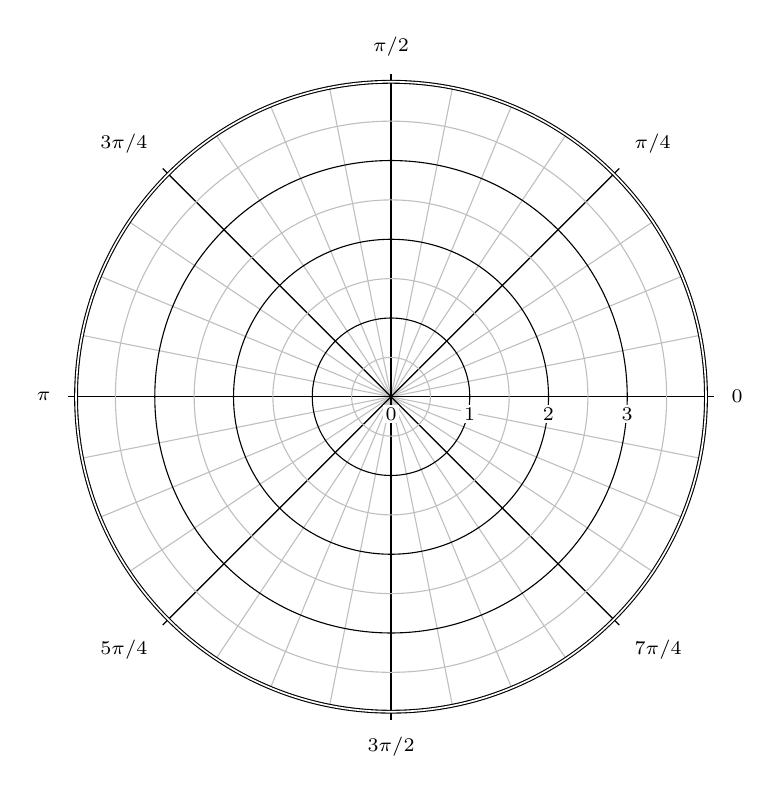
\begin{tikzpicture}[>=latex,baseline=(current bounding box.north)]
        % Draw the lines at multiples of pi/12
        \foreach \ang in {0,...,31} {
          \draw [lightgray] (0,0) -- (\ang * 180 / 16:4);
        }
        
        % Add the labels at multiples of pi/4
        \foreach \ang/\lab/\dir in {
          0/0/right,
          1/{\pi/4}/{above right},
          2/{\pi/2}/above,
          3/{3\pi/4}/{above left},
          4/{\pi}/left,
          5/{5\pi/4}/{below left},
          7/{7\pi/4}/{below right},
          6/{3\pi/2}/below} {
          \draw (0,0) -- (\ang * 180 / 4:4.1);
          \node [fill=white] at (\ang * 180 / 4:4.2) [\dir] {\scriptsize $\lab$};
        }
        
        % Concentric circles and radius labels
        \foreach \s in {0, 1, 2, 3} {
          \draw [lightgray] (0,0) circle (\s + 0.5);
          \draw (0,0) circle (\s);
          \node [fill=white] at (\s, 0) [below=1mm,inner sep=1pt] {\scriptsize $\s$};
        }
        
        
        
        % The double-lined circle around the whole diagram
        \draw [style=double] (0,0) circle (4);
    \end{tikzpicture}
\end{minipage}

\begin{tcolorbox}[title= COORDINATE CONVERSION EQUATIONS ,colframe=black,sharp corners,colback=white,colbacktitle=white,coltitle=black]

    

    Let the point $P$ have polar coordinates $(r,\,\theta)$ and rectangular coordinates $(x,\,y)$. Then
    \begin{minipage}[t]{.45\linewidth}
        \[x=r\cos \theta\]
    \end{minipage}
    \hfill
    \begin{minipage}[t]{.45\linewidth}
        \[y=r\sin \theta\]
    \end{minipage}
    
    \begin{minipage}[t]{.45\linewidth}
        \[r^2=x^2+y^2\]
    \end{minipage}
    \hfill
    \begin{minipage}[t]{.45\linewidth}
        \[\tan\theta=\frac{y}{x}\]
    \end{minipage}
    
\end{tcolorbox}
\vspace{.1cm}
\noindent\textbf{Examples:} Convert the following points/equations to the other coordinate system.
\begin{questions}
    \begin{minipage}{.45\linewidth}
        \question $\displaystyle\left(2,\,\frac{5\pi}{6}\right)$
    \end{minipage}
    \hfill
    \begin{minipage}{0.45\linewidth}
        \question $\displaystyle (3,\,-3)$
    \end{minipage}
    
    \newpage
    
    \begin{minipage}{0.45\linewidth}
        \question $y=4$
    \end{minipage}
    \hfill
    \begin{minipage}{0.45\linewidth}
        \question $x^2+y^2=25$
    \end{minipage}
    
    \vspace{\stretch{1}}
    
    \begin{minipage}{0.45\linewidth}
        \question $r\sin\theta=3$
    \end{minipage}
    \hfill
    \begin{minipage}{0.45\linewidth}
        \question $\displaystyle\theta=\frac{2\pi}{3}$
    \end{minipage}

    \vspace{\stretch{1}}    
    
\end{questions}

\textbf{Graphing:}
\begin{questions}
    \begin{minipage}{0.45\linewidth}
        \question $r=2\cos3\theta$\\
        \\
        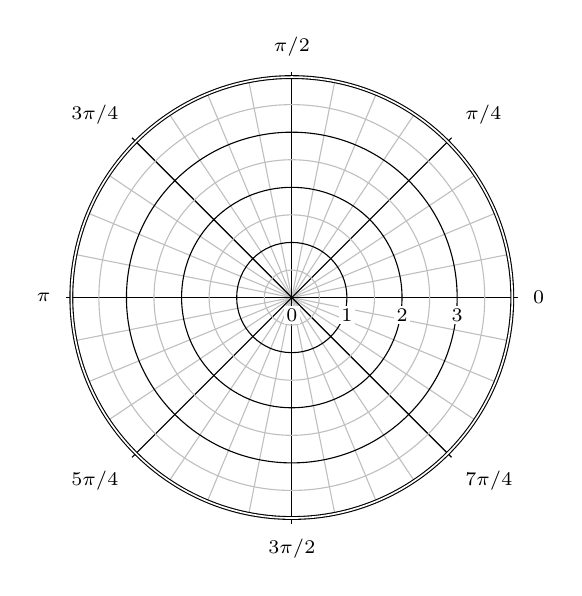
\begin{tikzpicture}[>=latex,baseline=(current bounding box.north),scale=.7]
            % Draw the lines at multiples of pi/12
            \foreach \ang in {0,...,31} {
              \draw [lightgray] (0,0) -- (\ang * 180 / 16:4);
            }
            
            % Add the labels at multiples of pi/4
            \foreach \ang/\lab/\dir in {
              0/0/right,
              1/{\pi/4}/{above right},
              2/{\pi/2}/above,
              3/{3\pi/4}/{above left},
              4/{\pi}/left,
              5/{5\pi/4}/{below left},
              7/{7\pi/4}/{below right},
              6/{3\pi/2}/below} {
              \draw (0,0) -- (\ang * 180 / 4:4.1);
              \node [fill=white] at (\ang * 180 / 4:4.2) [\dir] {\scriptsize $\lab$};
            }
            
            % Concentric circles and radius labels
            \foreach \s in {0, 1, 2, 3} {
              \draw [lightgray] (0,0) circle (\s + 0.5);
              \draw (0,0) circle (\s);
              \node [fill=white] at (\s, 0) [below=1mm,inner sep=1pt] {\scriptsize $\s$};
            }
            
            
            
            % The double-lined circle around the whole diagram
            \draw [style=double] (0,0) circle (4);
        \end{tikzpicture}
    \end{minipage}
    \hfill
    \begin{minipage}{0.45\linewidth}
        \question $r=2(1-\cos\theta)$\\
        \\
        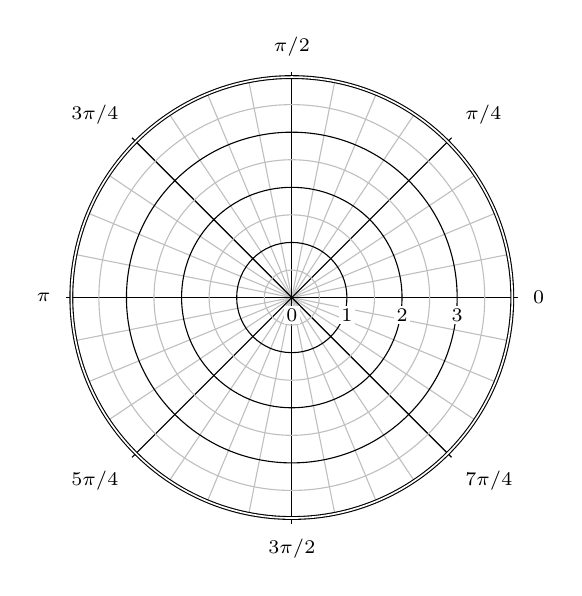
\begin{tikzpicture}[>=latex,baseline=(current bounding box.north),scale=.7]
            % Draw the lines at multiples of pi/12
            \foreach \ang in {0,...,31} {
              \draw [lightgray] (0,0) -- (\ang * 180 / 16:4);
            }
            
            % Add the labels at multiples of pi/4
            \foreach \ang/\lab/\dir in {
              0/0/right,
              1/{\pi/4}/{above right},
              2/{\pi/2}/above,
              3/{3\pi/4}/{above left},
              4/{\pi}/left,
              5/{5\pi/4}/{below left},
              7/{7\pi/4}/{below right},
              6/{3\pi/2}/below} {
              \draw (0,0) -- (\ang * 180 / 4:4.1);
              \node [fill=white] at (\ang * 180 / 4:4.2) [\dir] {\scriptsize $\lab$};
            }
            
            % Concentric circles and radius labels
            \foreach \s in {0, 1, 2, 3} {
              \draw [lightgray] (0,0) circle (\s + 0.5);
              \draw (0,0) circle (\s);
              \node [fill=white] at (\s, 0) [below=1mm,inner sep=1pt] {\scriptsize $\s$};
            }
            
            
            
            % The double-lined circle around the whole diagram
            \draw [style=double] (0,0) circle (4);
        \end{tikzpicture}
    \end{minipage}
\end{questions}
    
    


\newpage
